% -*- Mode: latex -*- %


\subsection{A few motivating examples}
\label{sec:motivation-exp}


Standard validation methodology randomly splits data into
train/validation/test sets, artificially enforcing exchangeabilty).  Thus,
to motivate the challenges in predictive validity even
under simple covariate shifts---we only modify the
distribution of $X$, returning later to more sophisticated real-world
scenarios---we experiment on nine regression datasets from the UCI
repository~\cite{DuaGr17}. We repeat the following 50 times.  We randomly
partition each dataset into disjoint sets $D_\train, D_\val, D_\test$,
each consisting of $1/3$ of the data. We fit a random forest predictor $\mu$
using $D_\train$ and construct conformal intervals of the
form~\eqref{eqn:confidence-set} with $\score(x, y) = |\mu(x)- y|$, so that
$\what{C}_n(x) = \{y \mid |\mu(x) - y| \le \hat{t}\}$ for a threshold
$\hat{t}$ achieving coverage at nominal level $\alpha = .05$ on $D_\val$, as
is standard in split-conformal prediction~\cite{VovkGaSh05}.
We evaluate coverage on tiltings of varying strength on $D_\test$: letting
$v$ be the top eigenvector of the test $X$-covariance $\Sigma_\test$
and $\wb{x}_\test$ be the mean of $X$ over $D_\test$, we reweight $D_\test$
by probabilities proportional to $w(x) = \exp(a v^T (x -
\wb{x}_\test))$ for tilting parameters $a \in \pm \{0, .02, .04, .08, .16,
.32, .64\}$. Essentially, this shift asks the following question: why
would we \emph{not} expect a shift along the principal directions of
variation in $X$ on future data?

\begin{figure}[h!]
  \centering
  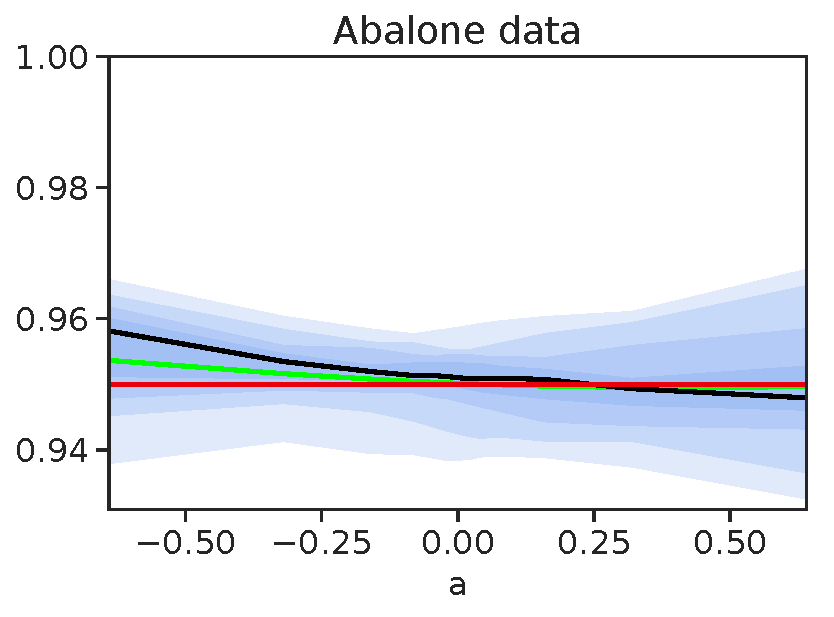
\includegraphics[width=0.3\linewidth]{uci/abalone_coverage_Standard_I-B.pdf}
  \hfill
  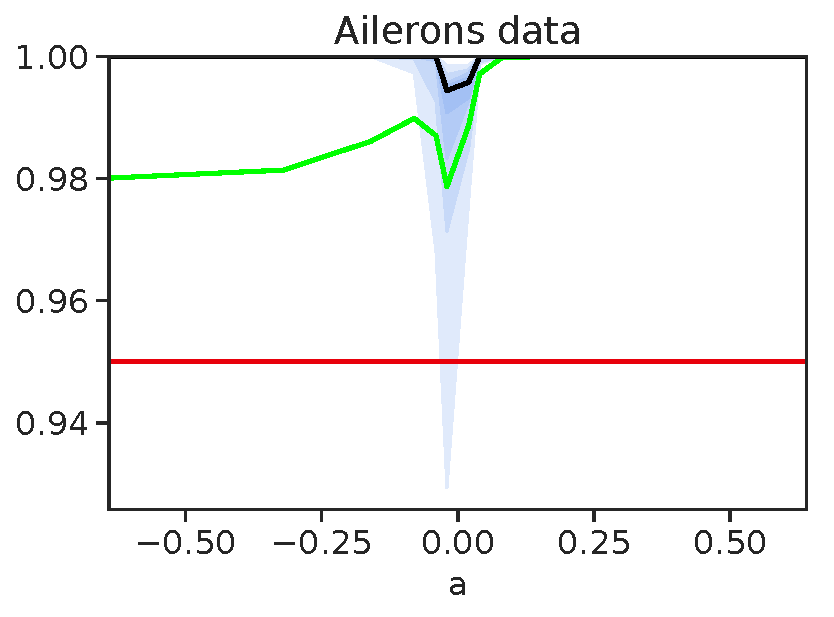
\includegraphics[width=0.3\linewidth]{uci/ailerons_coverage_Standard_I-B.pdf}
  \hfill
  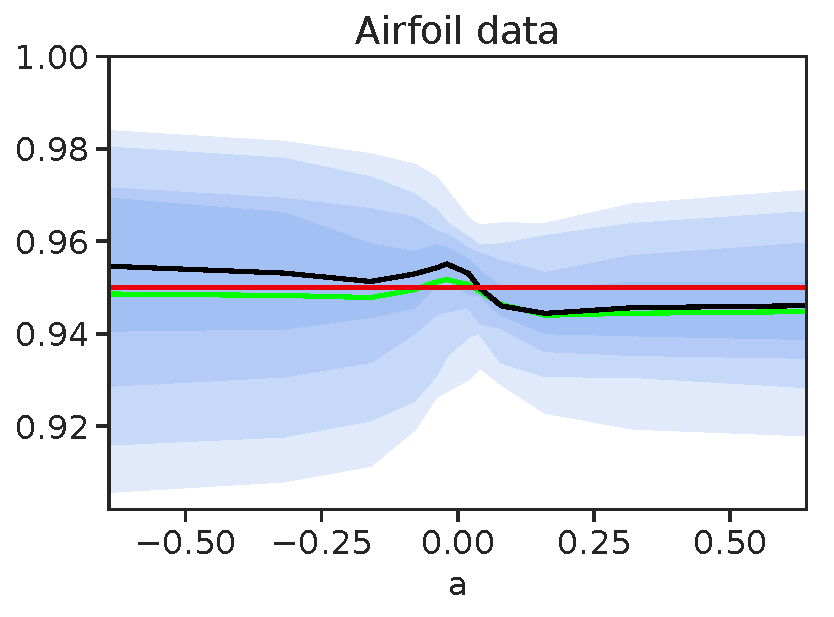
\includegraphics[width=0.3\linewidth]{uci/airfoil_coverage_Standard_I-B.pdf}
  \\
  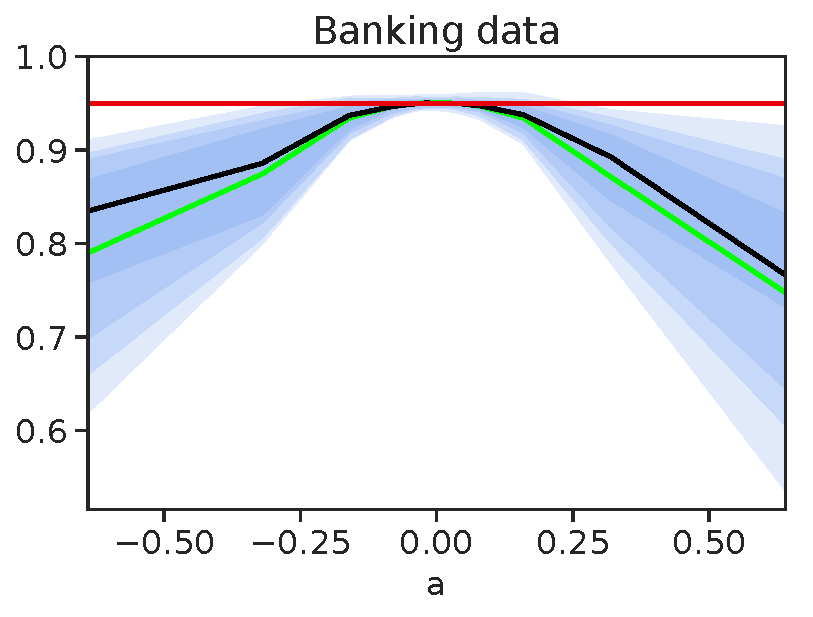
\includegraphics[width=0.3\linewidth]{uci/bank_coverage_Standard_I-B.pdf}
  \hfill
  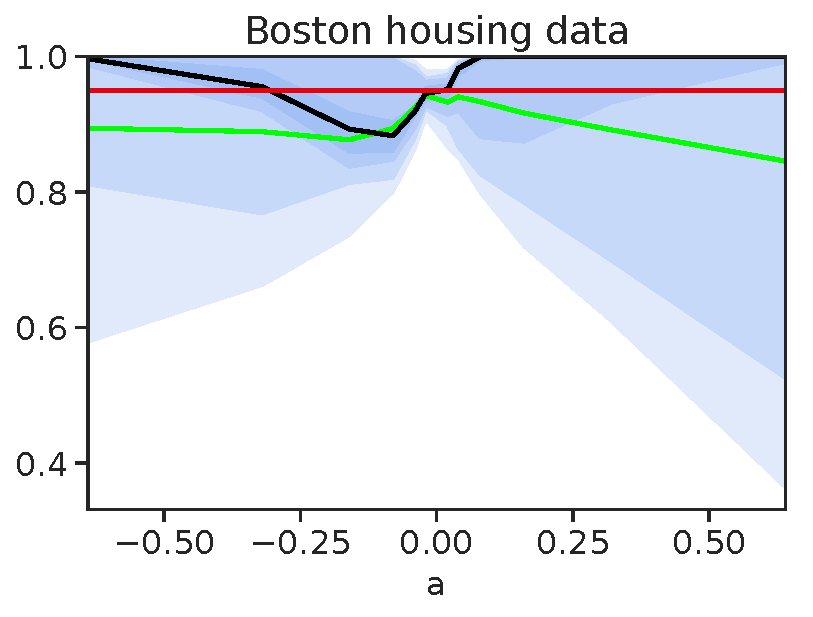
\includegraphics[width=0.3\linewidth]{uci/bos_coverage_Standard_I-B.pdf}
  \hfill
  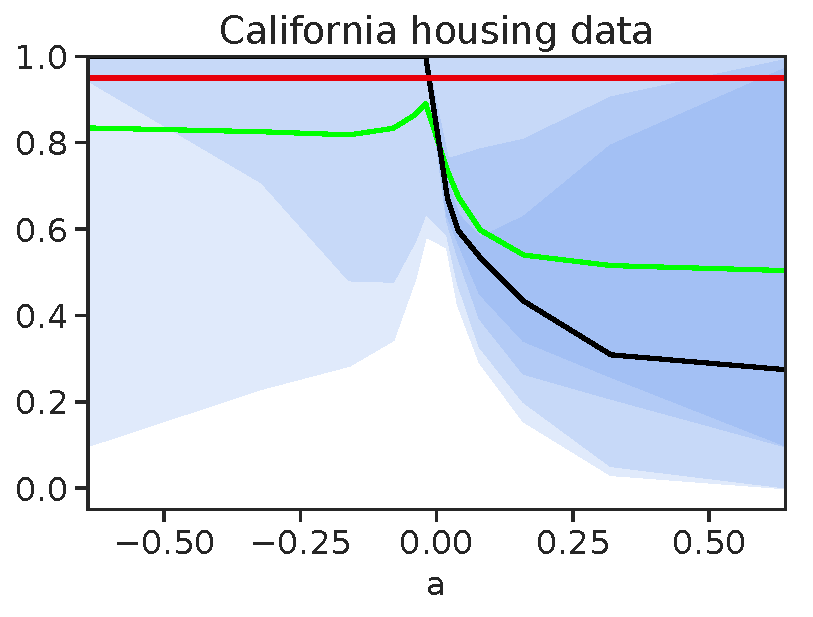
\includegraphics[width=0.3\linewidth]{uci/ca_coverage_Standard_I-B.pdf}
  \\
  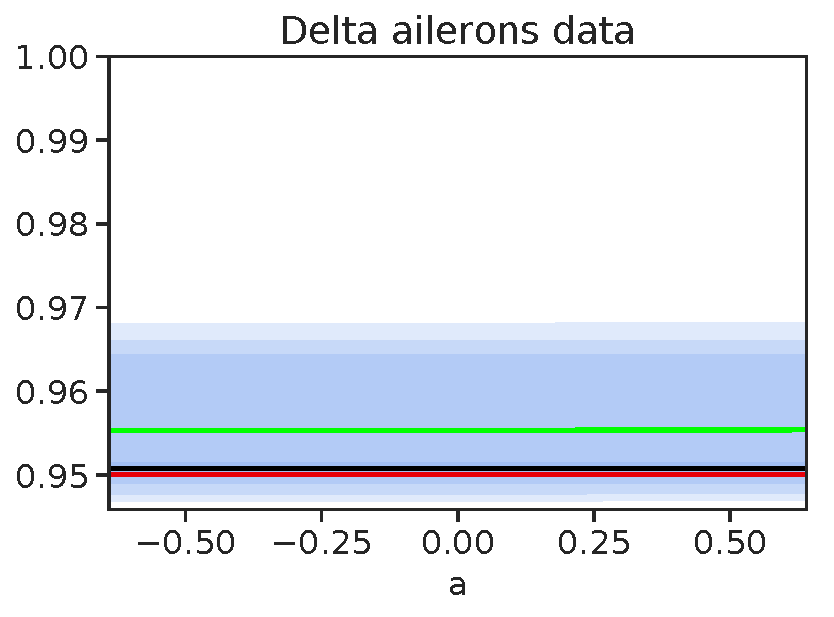
\includegraphics[width=0.3\linewidth]{uci/delta_coverage_Standard_I-B.pdf}
  \hfill
  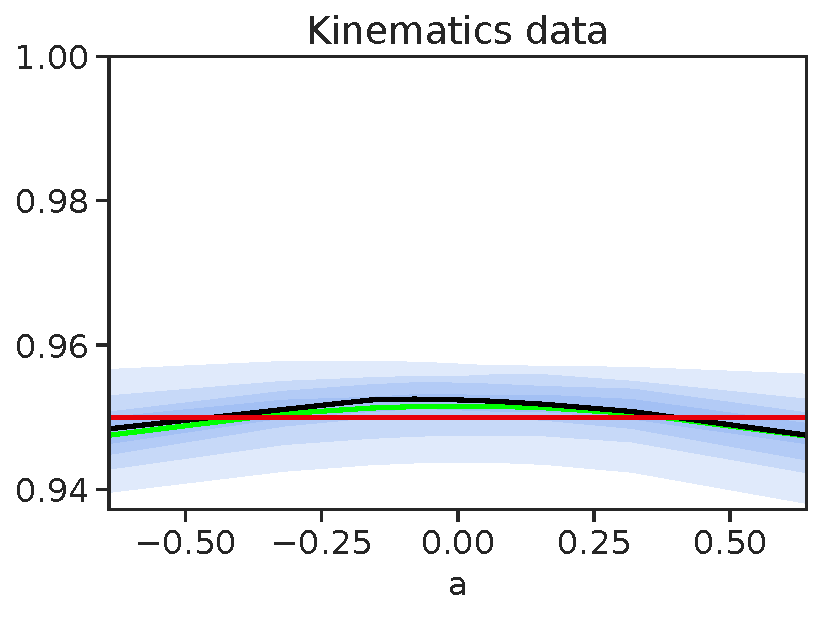
\includegraphics[width=0.3\linewidth]{uci/kin_coverage_Standard_I-B.pdf}
  \hfill
  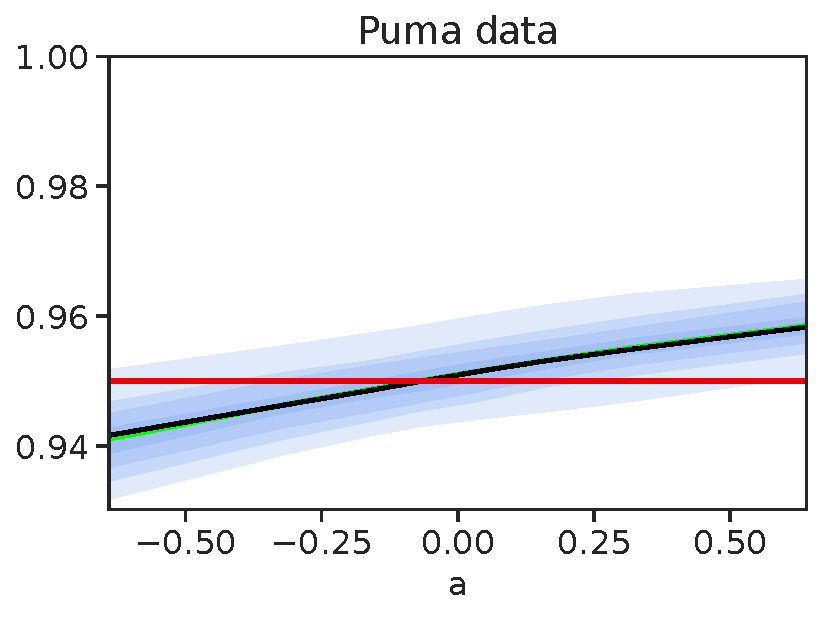
\includegraphics[width=0.3\linewidth]{uci/puma_coverage_Standard_I-B.pdf}  
  \caption{Empirical coverage for the prediction sets generated by the standard
    conformal methodology across nine regression data sets and 50
    random splits of each data set, with an exponential tilting in $X$ space
    along the first principal component of $X$. The horizontal axis gives the
    value of the tilting parameter $a$; the vertical the coverage level. A green
    line marks the average coverage, a black line marks the median coverage, and
    the horizontal red line marks the nominal coverage $.95$. The blue bands
    show the coverage at deciles over 50 splits.}
  \label{fig:cvgs_only_std}
\end{figure}

Figure~\ref{fig:cvgs_only_std} presents the results: even when the covariate
shifts are small, which corresponds to tilting parameters $a$ with small
magnitude, prediction intervals from the standard conformal methodology
frequently fail to cover (sometimes grossly) the true response values. While
this is but a simple motivation, if we expect some
shift in future data---say along the directions of principal variation in
$X$, as the data itself is already variable along that axis---it seems that
standard validation approaches~\cite{HastieTiFr09} provide too rosy
of a picture of future validity~\cite{RechtRoScSh19}, as they \emph{enforce}
exchangeability by randomly splitting data.
